\section{Computing Gross-Shape by Feature-based Defeaturing} \label{defeat}

In defeaturing of a feature-based CAD model, the relevance of each feature is measured by an evaluation metrics  \cite{AdskElectronicsHelp}.  The evaluation metrics used in this study is divided into two classes, viz. application context-specific criteria (Phase I) and geometric reasoning-based criteria (Phase II). This work focuses on the sheet metal domain as an example of application context-specific criteria for defeaturing, for the end-use of finding the gross shape needed for computing the midsurface. Fig. ref{fig} shows the overall process where Phase I is directly dependent on the feature information available in the sheet metal feature-based CAD models, and Phase II works on the final solid shape, while leveraging feature information for deciding the suppressibility.

%\begin{figure}[!ht]
%\RawFloats
\begin{minipage}[c]{0.58\linewidth}
\begin{itemize}
[noitemsep,topsep=2pt,parsep=2pt,partopsep=2pt,leftmargin=*]
\item \textbf{Phase I - Defeaturing based on the application context}: The model feature tree is traversed and the candidate features for suppression are identified based on certain criteria. In this study, rules based on the sheet metal features taxonomy are used to decide the suppressibility of the features. For other domains or applications, this phase can be customized by employing rules suitable to those applications.

\item \textbf{Phase II - Defeaturing based on geometric reasoning}: This phase starts with the final Brep for identifying the remnant portions of the features, and those whose sizes are below the threshold are identified for suppression. This phase, being geometric in nature, can be generic to different applications, with an option of customize the threshold based on engineering judgment appropriately.
\end{itemize}
    \end{minipage}
    \hfill
    \begin{minipage}[c]{0.4\linewidth}
        \centering
        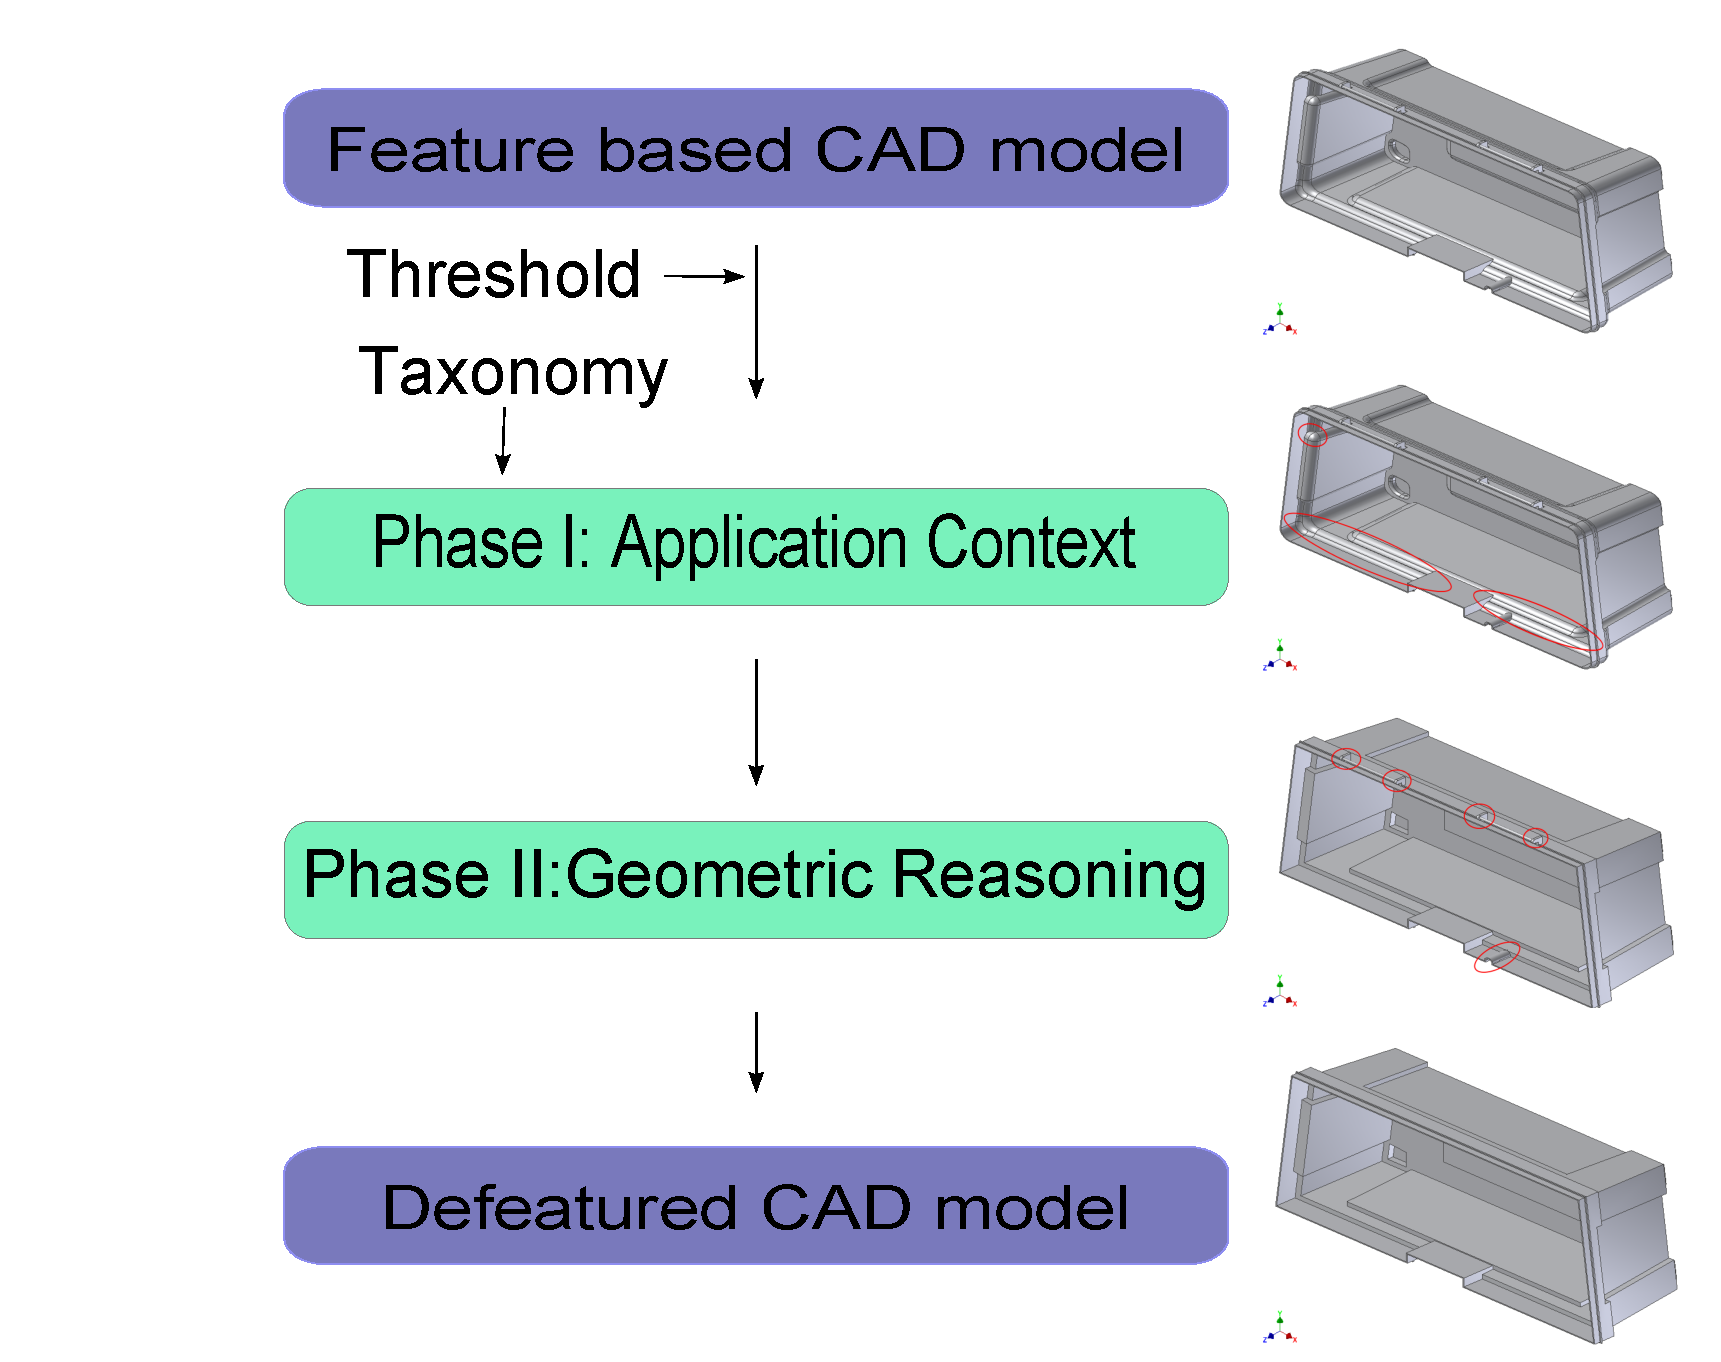
\includegraphics[width=\linewidth]{../Common/images/SystemArchitectureDefeat_1}
        \captionof{figure}{Overall Defeaturing Process}
        \label{fig:label}
    \end{minipage}
%\end{figure}

\bigskip

The combined method (Phase I \& II) is called as ``\textbf{Smarf}'' (\textbf{S}heet \textbf{M}etal and \textbf{R}emnant \textbf{F}eature). Following sections present the algorithms for both phases in details.


\subsection{Phase I: Defeaturing based on the application context}\label{ph1}

The case study shown in Table 1 shows effectiveness of the gross shapes in the generation of a better midsurface. The concept of "gross shape" is subjective and hard to quantify  \cite{LeeLee1998}. Thus formulating the rules for identification of suppressible features is the most critical step that affects the output of defeaturing. Apart from similar classifications in the literature, a thorough analysis of inputs from various surveys with engineers and experts on the field was done with respect to the midsurface quality metrics, such as preservation of medial-ness, problems, errors, etc.  Proposed  taxonomy (Figure ~\ref{fig:tax_sm}) is the result of this analysis. In comparison with the other sheet metal features classifications, such as for features recognition \cite{Gupta2013, Gupta2013a} and process planning \cite{Kannan2009} the proposed taxonomy is a novel one since the application context itself is different than the previous works.
%
%Sheet Metal parts are built using generic solid modeling features as well as some specialized sheet metal features. 
%

\subsubsection{Sheet Metal Features Taxonomy}\label{ph11}

Taxonomy is represented by “vocabulary” and “structure”. In the context of feature based CAD applications it is a scheme to represent and classify features for a particular purpose. In this paper sheet metal features are classified  (Fig ~\ref{fig:classification}) for the purpose of defeaturing as follows:

\bigskip

%\begin{tabular}[h]{@{} p{0.45\linewidth}  p{0.45\linewidth}@{}} 
\begin{minipage}[t]{0.45\linewidth}
\begin{itemize}
[noitemsep,topsep=2pt,parsep=2pt,partopsep=2pt]
\item \textbf{Primary Features}: These are not suppressed irrespective of their size as they form the principal/gross shape. Lacking these would create missing midsurface patches. Examples are:
	\begin{itemize} [noitemsep,topsep=2pt,parsep=2pt,partopsep=2pt]
	\item Face-Wall
	\item Flange
	\item Drawing
	\end{itemize}
\item \textbf{Secondary Features}: These are suppressed based on the relative size with respect to overall shapes and size-threshold. Smaller features unnecessarily create problems in geometric computation of midsurface, so they need to be suppressed.
 Examples are:
	\begin{itemize} [noitemsep,topsep=2pt,parsep=2pt,partopsep=2pt]
	\item Stamping
	\item Emboss 
	\end{itemize}
	
\item \textbf{Tertiary/Auxiliary Features}: They are not part of the main shape. So they can be suppressed irrespective of their sizes.
Examples are:
	\begin{itemize} [noitemsep,topsep=2pt,parsep=2pt,partopsep=2pt]
	\item Lip
	\item Rest 
	\end{itemize}
	
%\item \textbf{Connecting Features}: These are not suppressed irrespective of their sizes, as removing them, will create gaps between the sub-shapes of the original part. Lacking these would create gaps, so these are retained irrespective of their relative size, small or large.
%Example is:
%	\begin{itemize} [noitemsep,topsep=2pt,parsep=2pt,partopsep=2pt]
%	\item Bend
%	\end{itemize}
		
\item \textbf{Feature Groups}: Suppression criteria applied is evaluated on the collective group and not on individual feature. 	Examples are:
\begin{itemize} [noitemsep,topsep=2pt,parsep=2pt,partopsep=2pt]
	\item Mirror
	\item Patterns
	\end{itemize}
\end{itemize}

\end{minipage}
\hfill
\begin{minipage}[t]{0.52\linewidth}
\begin{minipage}[t]{\linewidth}
\dirtree{%
.1 Sheet Metal Features.
.2 Primary Features.
.3 Face-Wall   \adjustbox{valign=t}{
\includegraphics[scale=0.65]{..//Common/images/InventorWall.png}}.
.3 Flange  \quad \adjustbox{valign=t}{
\includegraphics[scale=0.65]{..//Common/images/InventorFlange.png}}.
.3 Bend   \qquad \adjustbox{valign=t}{
\includegraphics[scale=0.65]{..//Common/images/InventorBend.png}}.
%.3 Loft Flange  \qquad \adjustbox{valign=t}{
\includegraphics[scale=0.65]{..//Common/images/InventorLoftedFlange.png}}.
%.3 Rib \quad \quad  \adjustbox{valign=t}{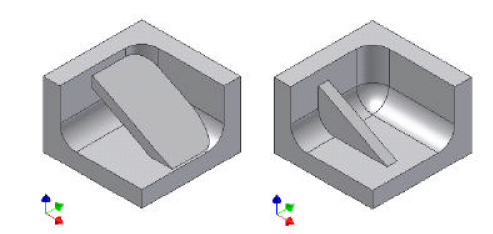
\includegraphics[height=0.11\linewidth]{..//Common/images/Feature_Rib.png}}.
.2 Secondary Features.
.3 Stamping  \quad \adjustbox{valign=t}{
\includegraphics[scale=0.65]{..//Common/images/InventorStamping.png}}.
.3 Cutout  \qquad \adjustbox{valign=t}{
\includegraphics[scale=0.65]{..//Common/images/InventorCutout.png}}.
%.3 Fold  \qquad \adjustbox{valign=t}{
\includegraphics[scale=0.65]{..//Common/images/InventorFold.png}}.
%.3 Roll  \qquad \adjustbox{valign=t}{
\includegraphics[scale=0.65]{..//Common/images/InventorRoll.png}}.
.3 Emboss \qquad \adjustbox{valign=t}{
\includegraphics[scale=0.65]{..//Common/images/InventorEmboss.png}}.
%.3 Hem   \quad \qquad \adjustbox{valign=t}{
\includegraphics[scale=0.65]{..//Common/images/InventorHem.png}}.
%.3 Grill \qquad \adjustbox{valign=t}{
\includegraphics[scale=0.65]{..//Common/images/InventorGrill.png}}.
.2 Tertiary/Auxiliary Features.
%.3 Chamfer \qquad \adjustbox{valign=t}{
\includegraphics[scale=0.65]{..//Common/images/InventorChamfer.png}}.
%.3 Round  \qquad \adjustbox{valign=t}{
\includegraphics[scale=0.65]{..//Common/images/InventorRound.png}}.
%.3 Thread \qquad \adjustbox{valign=t}{
\includegraphics[scale=0.65]{..//Common/images/InventorThread.png}}.
.3 Lip \qquad \adjustbox{valign=t}{
\includegraphics[scale=0.65]{..//Common/images/InventorLip.png}}.
.3 Rest \qquad \adjustbox{valign=t}{
\includegraphics[scale=0.65]{..//Common/images/InventorRest.png}}.
%.2 Connecting Features.
%.3 Bend   \qquad \adjustbox{valign=t}{
\includegraphics[scale=0.65]{..//Common/images/InventorBend.png}}.
.2 Features Groups.
.3 Mirror \quad  \quad \adjustbox{valign=t}{
\includegraphics[scale=0.65]{..//Common/images/InventorMirror.png}}.
%.3 RectPattern \quad  \adjustbox{valign=t}{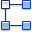
\includegraphics[scale=0.65]{..//Common/images/InventorRectPattern.png}}.
.3 Pattern\quad  \adjustbox{valign=t}{
\includegraphics[scale=0.65]{..//Common/images/InventorCircPattern.png}}.
}
\captionof{figure}{Sheet Metal features taxonomy (Icons source: \cite{Inventor2014Help})}\label{fig:tax_sm}
\end{minipage}
\bigskip
\begin{minipage}[t]{\linewidth}
\centering 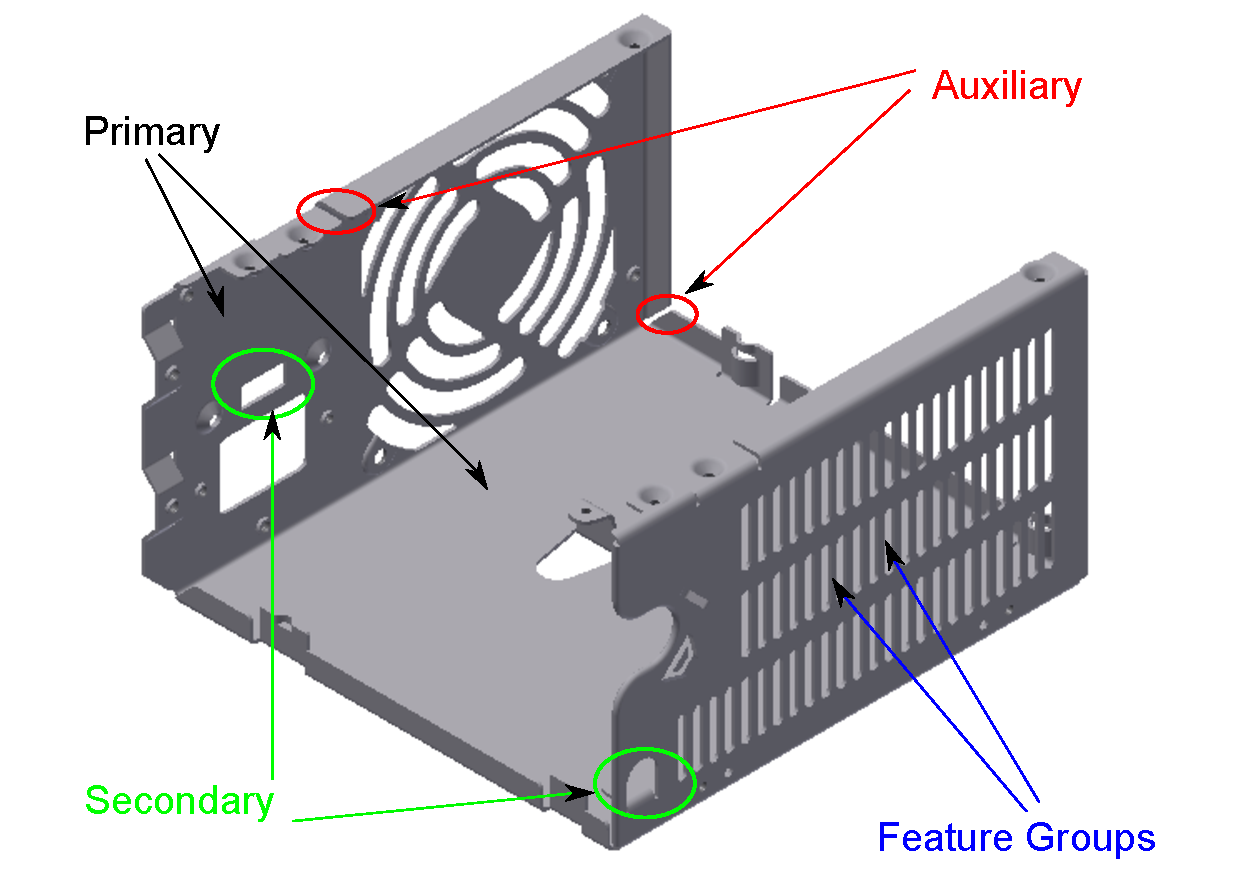
\includegraphics[width=0.8\linewidth]{..//Common/images/SheetMetal_taxonomy.pdf}
\captionof{figure}{Examples of classified types}\label{fig:classification}
\end{minipage}
\end{minipage}

Examples of these features are presented in a sheet metal part model as shown in Fig.  \ref{fig:classification}.

\subsubsection{Defeaturing Sheet Metal model}

The following steps identify the sheet metal features as per the classification presented in section \ref{ph11}.
The identification uses the feature tree available as part of the feature based CAD model.

\bigskip

{\em Algorithm to identify candidate features for de-featuring based on Sheet Metal feature taxonomy:}

\begin{minipage}[c]{0.55\linewidth}
\begin{itemize}
[noitemsep,topsep=2pt,parsep=2pt,partopsep=2pt,leftmargin=*]

\item A List  ({\bf $sl$}) initialized to which the suppressible features are added. 
\item The model feature tree is traversed and the candidate features for suppression are identified based on a set of heuristic criteria such as ``Primary features are not to be suppressed'', ``Secondary features, if small, are selected'' etc.  (Figure \ref{fig:tax_sm}).
\item The identified features are added to {\bf $sl$}.
\item The {\bf $sl$} is presented to the user for verification and changes, if necessary. 
\item Features in  {\bf $sl$} are suppressed.
\item The model is regenerated and Defeaturing Effectiveness is computed using Eqn. \ref{val}
\end{itemize}
 
\end{minipage}
\hfill
\begin{minipage}[c]{0.43\linewidth}
\centering 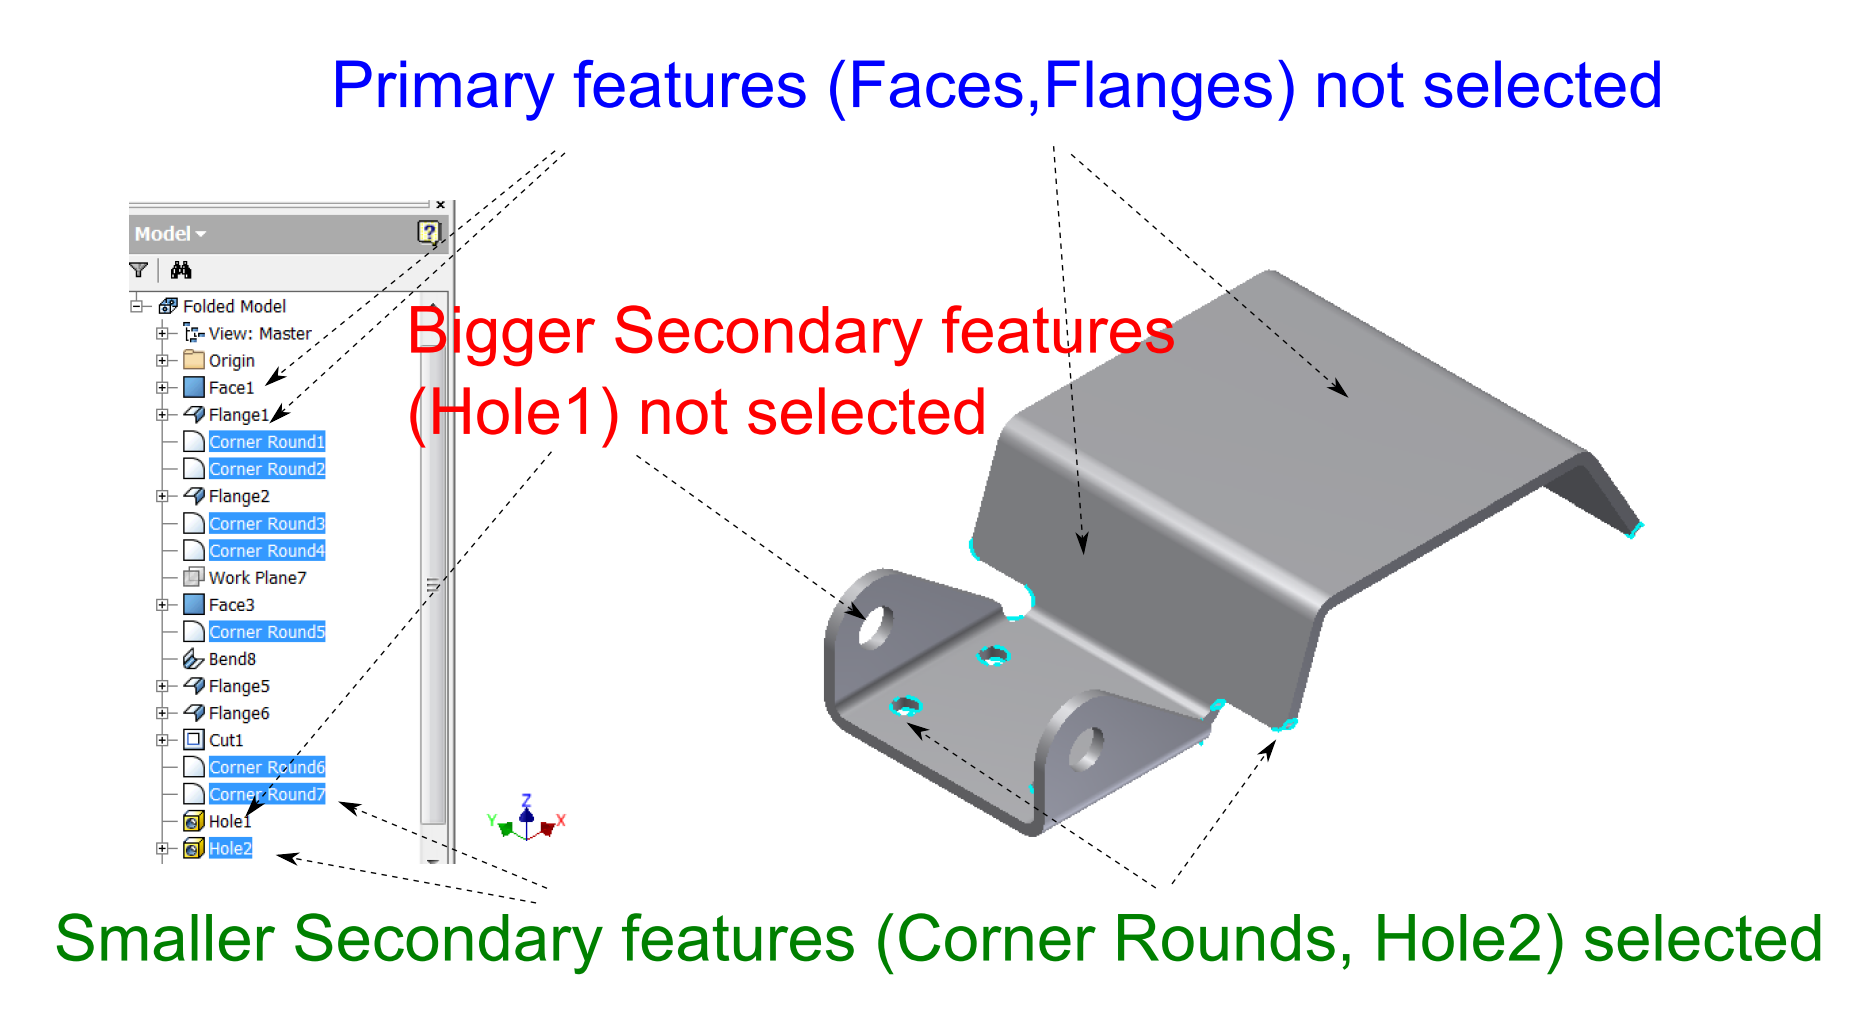
\includegraphics[width=\linewidth]{..//Common/images/SheetMetal_Ph1_Selection_Annotated}
\captionof{figure}{Examples of classified types}\label{fig:classification}
\end{minipage}

\subsubsection{Phase I: Algorithm 1}


\begin{algorithm}[!h]
	\caption{Application context-specific – Sheet metal features}
	\label{alg1}
	\begin{algorithmic}
		\REQUIRE A CAD model with access to the feature tree
		\WHILE{$nextFace() != null$}
			\STATE $F_i = currentFace()$
			\STATE $Area_{face} \quad += F_i \rightarrow area()$
		\ENDWHILE		
		\STATE $p = getInputFromUser()$
		\STATE $D = \frac{p}{100} \times Area$  \hspace{60mm} //threshold size
		\WHILE{$nextFeature() != null$}
			\STATE $f_i = currentFeature()$
			\IF {$f_i \rightarrow isAncillaryFeature()$}
				\STATE $sl \rightarrow add(f_i)$
			\ELSIF {$f_i \rightarrow isGroupFeature()$}
			  	\STATE $Area_{feature} = f_i \rightarrow combinedArea()$ \hspace{20mm}  // Total area of the constituent features
			  	\IF {$Area_{feature}< D$}
			  		\STATE $sl \rightarrow add(f_i)$
				\ENDIF
			\ELSE
				\STATE size $Area_{feature} = f_i \rightarrow area()$
			  	\IF {$Area_{feature} < D$}
			  		\STATE $sl \rightarrow add(f_i)$
				\ENDIF				
			\ENDIF
		\ENDWHILE
		\STATE  $sl \rightarrow suppress()$
		\STATE  $validate()$
	\end{algorithmic}
\end{algorithm}

\subsubsection{Results of Phase I}

The Phase I process is shown pictorially below. The first picture of Fig. \ref{fig:phaseI}

\begin{minipage}[t]{\linewidth}
\begin{tabular}[h]{@{} p{0.3\linewidth} p{0.3\linewidth}  p{0.3\linewidth}@{}} \toprule

\textbf{Input model to Phase I} & \textbf{Selected sheet metal features} & \textbf{Output of Phase I} \\ \midrule

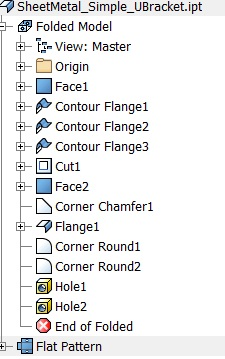
\includegraphics[width=0.92\linewidth]{..//Common/images/DefeatPhase_I_t1} &
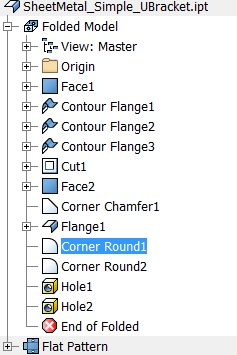
\includegraphics[width=0.98\linewidth]{..//Common/images/DefeatPhase_I_t2} &
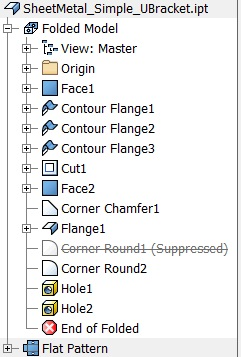
\includegraphics[width=0.99\linewidth]{..//Common/images/DefeatPhase_I_t3} \\ \midrule

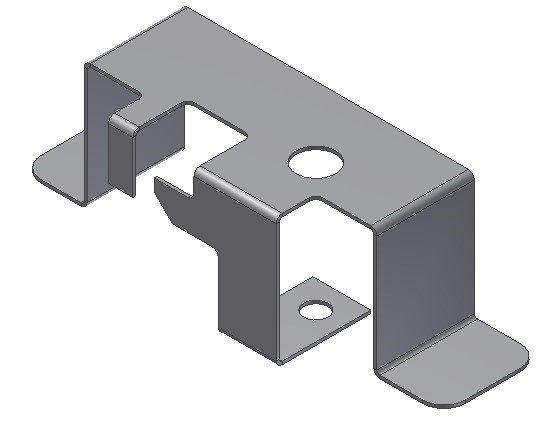
\includegraphics[width=0.98\linewidth]{..//Common/images/DefeatPhase_I_1} &
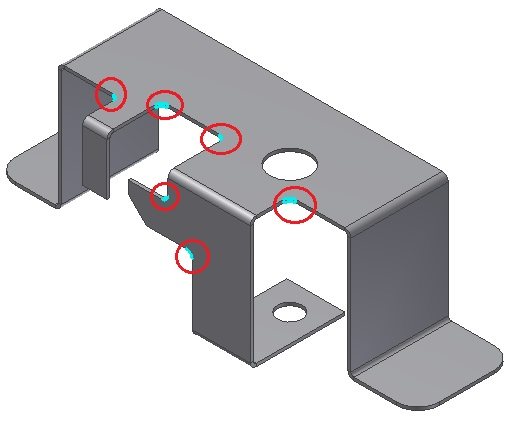
\includegraphics[width=0.98\linewidth]{..//Common/images/DefeatPhase_I_2} &
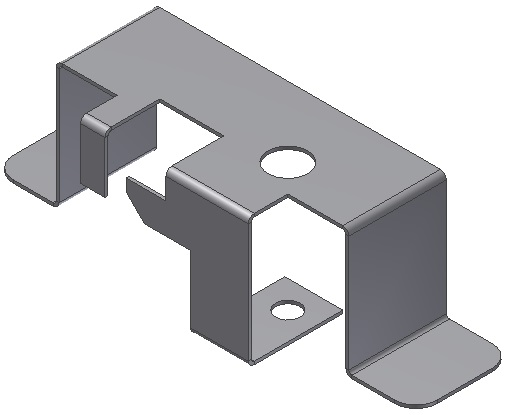
\includegraphics[width=0.98\linewidth]{..//Common/images/DefeatPhase_I_3} \\ \bottomrule

\end{tabular}
\captionof{figure}{Phase I}\label{fig:phaseI}
\end{minipage}

%\vspace{-3mm}


 %\vspace{-5mm}
 
\subsection{Phase II: Defeaturing based on Geometric Reasoning} \label{ph2}

In the feature-based design paradigm, the CAD model is built step-by-step using features at each step. Feature parameters are used to compute the ‘canonical’ (tool-body) volume first, which is then booleaned to the model built till then. During this operation, some portion of the canonical volume may get consumed, leaving behind the remaining (remnant) volume in the final solid  (Fig.~\ref{fig_remnant}).

\begin{figure}[!htb]
\centering
 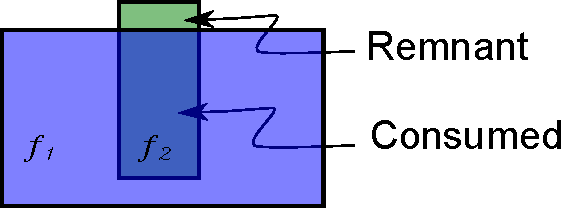
\includegraphics[width=0.35\linewidth]{../Common/images/Solid_Simple_SmallProtrusion.pdf} 
 \caption{Remnant and Consumed portions of feature volume of  $f_2$}
 \label{fig_remnant}
\end{figure}
  
Identification of suppressible features based on the feature volume computed from the full feature parameters yield incorrect results as the final shape may not retain the full feature volume. So, this work has devised a novel method  (Algorithm \ref{alg2}) to find the size of remnant feature volume to be used for deciding the suppressibility  (Fig.~\ref{fig:phaseII}) of the features.

This phase starts with the final Brep for identifying the remnant portions of the features. This computation, being geometric in nature, can be generic to many applications, with an option to customize the threshold based on engineering judgment specific to the given application.

\subsubsection{Preliminaries}
\begin{itemize}
[noitemsep,topsep=2pt,parsep=2pt,partopsep=2pt]
\item At $j^{th}$ feature ($f_j$), the model built till then is referred as $M_{j-1}$.  
\item $V_j = volume (f_j)$. $V_j$ is the feature/canonical/tool-body volume of the feature $f_j$.
\item $M_j = M_{j-1} \bigoplus V_j$. The model moves to the next state $M_j$ by boolean of existing state $M_{j-1}$ with the feature volume $f_j$ i.e. $V_j$. 
\item $V_j = R_{j} \cup C_j$. Some portion of $V_j$ gets consumed ($C_j$) and some remains ($R_j$). (Fig.~\ref{fig_remnant})
\item $M_j = M_{j-1} \cup  R_j$ and thus $R_j = M_{j} -   M_{j -1}$ is the remnant feature volume  \cite{Lee2005}.
\end{itemize} 

\bigskip

{\em Algorithm to identify candidate features for de-featuring based on Remnant Feature method:}
\begin{itemize}
[noitemsep,topsep=2pt,parsep=2pt,partopsep=2pt]
\item Faces of the final body are iterated. 
\item For each remnant face, its owning feature is extracted via attributes stored on them. 
\item Clusters/Groups of faces are built based on the owning features as shown in Fig. \ref{fig_clusters}. The dotted portion in a cluster represents the Consumed Feature, whereas the encircled portion is the Remnant feature



  \begin{minipage}{0.8\textwidth}

\begin{minipage}[c]{0.48\linewidth}
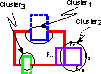
\includegraphics[width=0.7\linewidth]{../Common/images/clusters.pdf} 
\captionof{figure}{Formation of clusters} \label{fig_clusters}
\end{minipage}
\hfill
\begin{minipage}[c]{0.48\linewidth}
\begin{tabular}[h]{@{} p{0.3\linewidth} p{0.3\linewidth} p{0.3\linewidth}@{}} \toprule
\textbf{Clusters} & \textbf{Size}& \textbf{Feature}\\ \midrule
luster$_1$ & 0.25 	&  Extrude$_2$\\
luster$_2$ & 0.25  & Extrude$_3$\\
luster$_3$ & 0.125 & Hole$_1$\\ \bottomrule
%$f_{10}, f_{12}, f_{15}, f_{14}$ 	& Cluster$_4$\\ \bottomrule
\captionof{table}{ Evaluating Cluster sizes}
\label{tbl_clusters}
\end{tabular}
\end{minipage}
\end{minipage}
\vskip 4mm
\item Size of the cluster can be calculated by various methods like Influence Volume (obtained as a difference of the volume, if the feature is suppressed and then unsuppressed) or the union of bounding-boxes, etc. This work uses summation of the area of the remnant faces (Tab. \ref{tbl_clusters}) as the Size criterion.
\item Each cluster-owning feature(s) is added to {\em sl} based on the threshold value given by the user.
\item The {\em sl}  is presented to the user for verification and changes, if necessary. 
\item Features in {\em sl} are suppressed.
\item The model is regenerated and Defeaturing Effectiveness is computed (section \ref{effect}).
\end{itemize} 

\subsubsection{Phase II: Algorithm 2}

\begin{algorithm}[!tbh]
	\caption{Remnant Faces method}
	\label{alg2}
	\begin{algorithmic}
		\REQUIRE A CAD model with access to the feature tree. 
		\WHILE{$nextFace() != null$}  
			\STATE $F_i = currentFace()$
			\STATE $feat = F_i \rightarrow owingFeature()$
			\STATE $addedFlag = false$
			\WHILE {$nextCluster() != null$}
				\STATE $cl_j = currentCluster()$
				\IF {$cl_j \rightarrow owingFeature() == feat$}
					\STATE  $cl_j \rightarrow add(F_i)$
					\STATE $addedFlag = true$
				\ENDIF
			\ENDWHILE
			\IF {$addedFlag == false$}
				\STATE  $cl_n = newCluster()$
				\STATE  $cl_n \rightarrow owingFeature() = feat$
				\STATE  $cl_n \rightarrow add(f_i)$
			\ENDIF
		\ENDWHILE
		\WHILE {$nextCluster() != null$}
			\STATE $cl_k = currentCluster()$
			\STATE $size = cl_k \rightarrow calculateSize()$
			\IF {$size < D$} %\hspace{40mm} // Threshold ‘D’ defined in Alg \ref{alg1}
				\STATE   $sl \rightarrow add(cl_k)$
			\ENDIF			
		\ENDWHILE
		\STATE  $sl \rightarrow suppress()$
		\STATE  $validate()$
	\end{algorithmic}
\end{algorithm}

\bigskip
\subsubsection{Results of Phase II}

The Phase II process is shown pictorially in Fig. \ref{fig:phaseII}

\begin{itemize}
[noitemsep,topsep=2pt,parsep=2pt,partopsep=2pt]
\item The first picture shows input to this phase (it is the output of the previous Phase I)
\item The second picture shows the features selected by the remnant feature method, and 
\item The last picture shows the defeatured model as output of the Phase II.
\end{itemize}

\begin{minipage}[t]{\linewidth}
\begin{tabular}[h]{@{} p{0.3\linewidth} p{0.3\linewidth}  p{0.3\linewidth}@{}} \toprule

\textbf{Input model to Phase II} & \textbf{Selected Remnant method} & \textbf{Output of Phase II} \\ \midrule

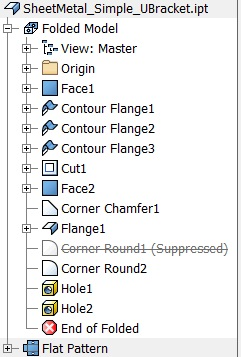
\includegraphics[width=0.92\linewidth]{..//Common/images/DefeatPhase_II_t1} &
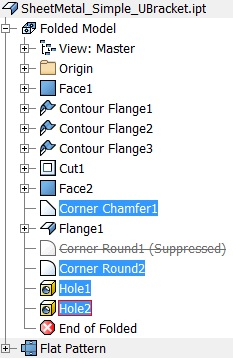
\includegraphics[width=0.98\linewidth]{..//Common/images/DefeatPhase_II_t2} &
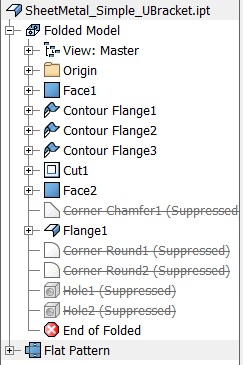
\includegraphics[width=0.99\linewidth]{..//Common/images/DefeatPhase_II_t3} \\ \midrule

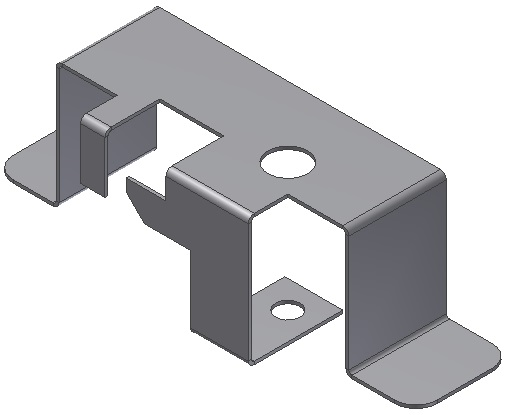
\includegraphics[width=0.98\linewidth]{..//Common/images/DefeatPhase_I_3} &
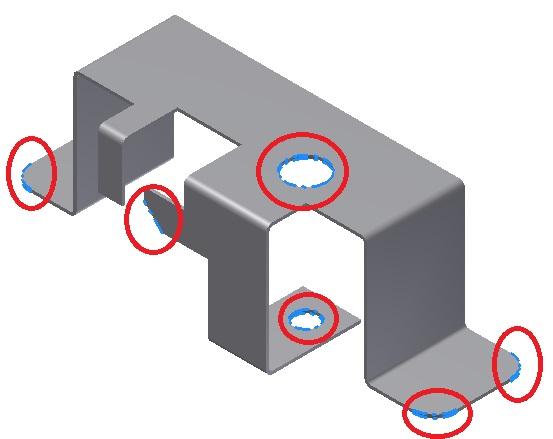
\includegraphics[width=0.98\linewidth]{..//Common/images/DefeatPhase_II_2} &
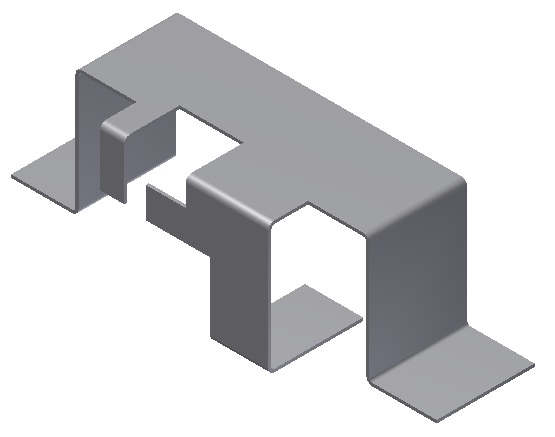
\includegraphics[width=0.98\linewidth]{..//Common/images/DefeatPhase_II_3} \\ \bottomrule

\end{tabular}
\captionof{figure}{Phase II}\label{fig:phaseII}
\end{minipage}

Output of Phase II (Fig. \ref{fig:phaseII}) is the gross shape of the input given (Fig. \ref{fig:phaseI}). With 50\% reduction in the number of features and 17\% reduction in the number of faces, the gross shape resulted has retained all the important features necessary for the computation of a well-connected midsurface.

\subsection{Effectiveness of Defeaturing}\label{effect}
Effectiveness of the defeaturing process can be computed using a wide variety of methods. They can be classified into input-based and output-based methods. In the input-based method, based on the engineering judgment, the initial defeaturing parameters (such as, size threshold, feature taxonomy, etc.) are set, and the output resulted is considered as the valid one. In the output-based method, some initial defeaturing parameters are set and the output is assessed against desired benchmarks, such as, reduction in volume/faces/features, etc. The process is repeated till the desired output is achieved. In this work, the effectiveness of defeaturing is computed by measuring {\bf Percentage reduction in the number of the faces}. More the percentage, the more effective is the defeaturing process. Features can also be used in place of faces to form another criterion for measuring the effectiveness:

	\begin{enumerate}
	[noitemsep,topsep=2pt,parsep=2pt,partopsep=2pt]
%	\item Total area of the Faces ($aF$)  ($mm^2$) 
%	\item Threshold size is some (say, 5 percent) of $aF$ ($sP$ $mm^2$)
	\item Total number of the faces in the original part ($nF$)
	\item Number of sheet metal features suppressed in Phase I ($nS$)
	%\item Time spent in detecting the suppressible features in Phase I ($tS$ sec) 
	\item Number of faces left after Phase I ($mF$)
	\item Number of generic features suppressed in Phase II ($nR$)
	%\item Time spent in detecting the suppressible features in Phase II ($tR$ sec)	
	\item Number of faces left after Phase II ($rF$)
	\item Defeaturing effectiveness ($pR$) while keeping the overall shape intact (\%)
	\begin{equation}\label{val}  pR = (1 - \frac{rF}{nF}) \times 100\end{equation}
	\end{enumerate}

Apart from $pR$, there could be some other and more involved criteria that can be used as follows:
	\begin{itemize}
	[noitemsep,topsep=2pt,parsep=2pt,partopsep=2pt]
	\item \textbf{Medial Axis Comparisons}: Small features create branches in their Medial Axis Transform (MAT \cite{Ramanathan2004})  representation. So, a complex model will have branches and its corresponding defeatured model won't have them. Comparison of both can give idea about the effectiveness.
	\item \textbf{Mesh}: Comparing faceted mesh generated by body defeatured by {\bf Smarf} with the mesh simplified by any benchmark mesh simplification methods can give the effectiveness measure.
	\item \textbf{Size}: Comparison of volume of the original and the defeatured model.
	\item \textbf{Shape deviation}: Using Part-Compare functionality, maximum deviation between the original and the defeatured, can be calculated. This deviation should be within predefined limits.
\end{itemize}



